\section{Methodology}\label{sec:methodology}

Th problem defined in section \ref{sec:model_overview} describes a normal-form
game between the decision makers of two queueing systems and a third player that 
decides how to distribute individuals to the systems.
The strategy space of the two queueing systems is defined as the possible values
that the threshold parameter can take \(T_i \in (1, N_i)\).
Then, the distributor has to decide on the proportion of individuals to send to 
each queueing system \(p_A \text{ and } p_B\), where \(p_A, p_B \in [0, 1] \)
and \(p_A + p_B = 1\).
Figure \ref{fig:imperfect-info-game} shows a diagrammatic 
representation of the game to be played and the decisions to be made.

\begin{figure}[ht]
    \centering
    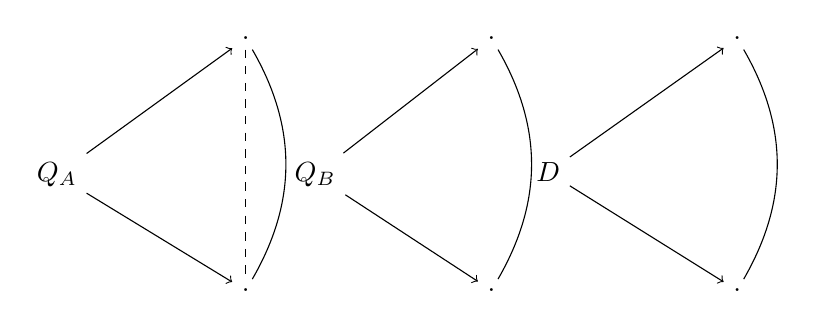
\begin{tikzpicture}[-, node distance = 3cm, scale=0.8]
        \node[anchor=north](HA){\(Q_A\)};
        \node[anchor=north](HA_d1) at (3, 2){.};
        \node[anchor=north](HA_d2) at (3, -2){.};
    
        \path[->] (HA) edge node {}(HA_d1);
        \path[->] (HA) edge node {}(HA_d2);
        \path (HA_d1) edge [bend left] node {}(HA_d2);
        \path (HA_d1) [dashed] edge node {}(HA_d2);
    
        \node[anchor=north](HB) at (4.1, 0){\(Q_B\)};
        \node[anchor=north](HB_d1) at (6.9, 2){.};
        \node[anchor=north](HB_d2) at (6.9, -2){.};
    
        \path[->] (HB) edge node {}(HB_d1);
        \path[->] (HB) edge node {}(HB_d2);
        \path(HB_d1) edge [bend left] node {}(HB_d2);
    
        \node[anchor=north](D) at (7.8, 0){\(D\)};
        \node[anchor=north](D_d1) at (10.8, 2){.};
        \node[anchor=north](D_d2) at (10.8, -2){.};
        
        \path[->] (D) edge node {}(D_d1);
        \path[->] (D) edge node {}(D_d2);
        \path(D_d1) edge [bend left] node {}(D_d2);
    \end{tikzpicture}
    \caption*{Figure 2 (revisited): Imperfect information Extensive Form Game 
    between the distributor and the 2 queueing systems}
\end{figure}

As described in section \ref{sec:model_overview} queueing system \(A\) decides
on a strategy, then queueing system \(B\) chooses its own threshold, unaware 
of the first queueing system's choice.
Finally, the distributor makes its choice based on the strategies that the 
queueing systems chose to play. 

The problem can be formulated by 3 matrices; the two payoff matrices of the 
normal form game and the routing matrix.
The payoff matrices and their utilities are defined by equations 
(\ref{eq:payoff-entry}) and (\ref{eq:payoff_matrices}) is section 
\ref{sec:model_overview}:

\begin{equation*}
    A = 
    \begin{pmatrix}
        U_{1,1}^A & U_{1,2}^A & \dots & U_{1,N_B}^A \\
        U_{2,1}^A & U_{2,2}^A & \dots & U_{2,N_B}^A \\
        \vdots & \vdots & \ddots & \vdots \\
        U_{N_A,1}^A & U_{N_A,2}^A & \dots & U_{N_A,N_B}^A \\
    \end{pmatrix},
    B = 
    \begin{pmatrix}
        U_{1,1}^B & U_{1,2}^B & \dots & U_{1,N_B}^B \\
        U_{2,1}^B & U_{2,2}^B & \dots & U_{2,N_B}^B \\
        \vdots & \vdots & \ddots & \vdots \\
        U_{N_A,1}^B & U_{N_A,2}^B & \dots & U_{N_A,N_B}^B \\
    \end{pmatrix}
    \tag{\ref{eq:payoff_matrices} revisited}
\end{equation*}


Similarly, the entries of the routing matrix are defined by equation 
(\ref{eq:obj_distributor}):
% TODO: Make sure this is defined PROPERLY and CONSISTENTLY in model_overview section or here in model_overview section or here
\begin{equation*}
    (p_A, p_B) \quad s.t. \quad 
    \alpha L_A(p_A) + (1 - \alpha) B_A(p_A) = 
    \alpha L_B(p_B) + (1 - \alpha) B_B(p_B)
    \tag{\ref{eq:obj_distributor} revisited}
\end{equation*}

Equation \ref{eq:obj_distributor} is properly defined and explained in section 
\ref{sec:model_overview}.
Thus, using equation \ref{eq:obj_distributor} for all possible sets of 
thresholds we can get the full routing matrix that consists of the proportions
to send to queueing system A (\(p_A\)) and to queueing system B (\(p_B\)).

\begin{equation}\label{eq:routing_matrix}
    R = 
    \begin{pmatrix}
        (p_{1,1}^A, p_{1,1}^B) & (p_{1,2}^A, p_{1,2}^B) & \dots & 
        (p_{1,N_B}^A, p_{1,N_B}^B) \\
        (p_{2,1}^A, p_{2,1}^B) & (p_{2,2}^A, p_{2,2}^B) & \dots & 
        (p_{2,N_B}^A, p_{2,N_B}^B) \\
        \vdots & \vdots & \ddots & \vdots \\
        (p_{N_A,1}^A, p_{N_A,1}^B) & (p_{N_A,2}^A, p_{N_A,2}^B) & \dots & 
        (p_{N_A,N_B}^A, p_{N_A,N_B}^B) \\
    \end{pmatrix}
\end{equation}

Note that since \(p_{i,j}^A + p_{i,j}^B = 1\) the routing matrix needs only to
store one of the two values; either \(p_{i,j}^A\) or \(p_{i,j}^B\).
Thus, the routing matrix \(R\) can be simplified to:

\begin{equation}\label{eq:routing_matrix_simplified}
    R = 
    \begin{pmatrix}
        p_{1,1}^A & p_{1,2}^A & \dots & p_{1,N_B}^A \\
        p_{2,1}^A & p_{2,2}^A & \dots & p_{2,N_B}^A \\
        \vdots & \vdots & \ddots & \vdots \\
        p_{N_A,1}^A & p_{N_A,2}^A & \dots & p_{N_A,N_B}^A \\
    \end{pmatrix}
\end{equation}

The game can thus be partitioned into a normal form game between the
two queueing systems and then finding the distributor's best strategy. 

\subsection{Backwards Induction}

In order to populate the payoff matrices and the routing matrix the method
of backwards induction is used.
Consider figure \ref{fig:imperfect-info-game} and the flow of the game that was
described (i.e. \(Q_A, Q_B \rightarrow D\)).
Due to the fact that the payoff matrices \(A\) and \(B\) depend on the routing 
matrix \(R\) the entries of the matrices are calculated in a backwards way 
(\(D \rightarrow Q_A, Q_B\)). 
Thus for every pair of strategies \(T_A, T_B\), the proportion of individuals 
that are to be transported to each queueing system is calculated first. 

Consider a game where the capacities of the two systems are \(N_A = 4\) and 
\(N_B = 3\).
The strategy space of players \(Q_A\) and \(Q_B\) would then be 
\(T_A = \{1, 2, 3, 4\}\) and \(T_B = \{1, 2, 3\}\) respectively.
Now, starting from an arbitrary starting point of \(T_A=1\) and \(T_B=1\), the
corresponding entry of the routing matrix the routing matrix can be calculated.
Using equation \ref{eq:obj_distributor} for \(T_A=1\) and \(T_B=1\):

\begin{equation*}
    (p_A, p_B) \quad s.t. \quad 
    \alpha L_A(p_A) + (1 - \alpha) B_A(p_A) = 
    \alpha L_B(p_B) + (1 - \alpha) B_B(p_B)
\end{equation*}

The above equation can be solved by using Brent's bisection algorithm.
% TODO: Cite Brent's algorithm
The calculated value of \(p_A\) corresponds to the entry on the first row and 
first column of the routing matrix:

\begin{equation}\label{eq:routing_matrix_1_1}
    R = 
    \begin{pmatrix}
        p_{1,1}^A & - & - \\
        - & - & - \\
        - & - & - \\
        - & - & - \\
    \end{pmatrix}
\end{equation}

In fact all remaining values of the routing matrix can be calculated by
solving \(N \times M\) similar equations using Brent's bisection algorithm.
Therefore, having calculated the entire routing matrix the payoff matrices can
be calculated.
Consider once again the case of \(T_A=1, T_B=1\). 

% TODO: Make sure this is defined PROPERLY and CONSISTENTLY in model_overview section or here
\begin{equation*}
    U_{1, 1}^A = \quad 1 -\left( 
        \hat{P} - P(W_A < R) 
    \right)^2,
    \quad
    U_{1, 1}^B = \quad 1 -\left( 
        \hat{P} - P(W_B < R) 
    \right)^2 \tag{\ref{eq:payoff-entry} revisited}
\end{equation*}

These are the utilities of players \(A\) and \(B\) when both players choose a
strategy of \(T = 1\).
% TODO: Change R everywhere to t
Here \(R\) is the predefined waiting time target to be met by a percentage of 
individuals \( \hat{P} \) and \(P(W_i < R)\) is properly defined in section
\ref{sec:proportion_within_target}.

\begin{equation}\label{eq:payoff_matrices_1_1}
    A = 
    \begin{pmatrix}
        U_{1, 1}^A & - & - \\
        - & - & - \\
        - & - & - \\
        - & - & - \\
    \end{pmatrix}, \quad
    B = 
    \begin{pmatrix}
        U_{1, 1}^B & - & - \\
        - & - & - \\
        - & - & - \\
        - & - & - \\
    \end{pmatrix}
\end{equation}

Similar to the routing matrix, the above procedure can be repeated for all 
possible values of \(T_A\) and \(T_B\) to populate all entries of the payoff 
matrices. 


\subsection{Nash Equilibrium}

\subsection{Learning Algorithms}
